\documentclass[10pt,aspectratio=169]{beamer}
\usepackage{tikz}
\usepackage[utf8]{inputenc}
%\usepackage[T1]{fontenc}
\usepackage[english]{babel}
%\usepackage[latin1]{inputenc}
%\usepackage[T1]{fontenc}
\usepackage{verbatim}
\usepackage{listings}

\lstset{
  language=C++,                 % the language of the code
  backgroundcolor=\color{white},   % choose the background color; you must add \usepackage{color} or \usepackage{xcolor}
  basicstyle=\footnotesize,        % the size of the fonts that are used for the code
  breakatwhitespace=false,         % sets if automatic breaks should only happen at whitespace
  breaklines=true,                 % sets automatic line breaking
  keywordstyle=\color{blue},       % keyword style
  captionpos=b,                    % sets the caption-position to bottom
  commentstyle=\color{blue},       % comment style
  deletekeywords={},            % if you want to delete keywords from the given language
  escapeinside={\%*}{*)},          % if you want to add LaTeX within your code
  extendedchars=true,              % lets you use non-ASCII characters; for 8-bits encodings only, does not work with UTF-8
  frame=single,                    % adds a frame around the code
  keepspaces=true,                 % keeps spaces in text, useful for keeping indentation of code (possibly needs columns=flexible)
  morekeywords={using, static_assert},            % if you want to add more keywords to the set
  numbers=left,                    % where to put the line-numbers; possible values are (none, left, right)
  numbersep=10pt,                   % how far the line-numbers are from the code
  numberstyle=\tiny\color{black}, % the style that is used for the line-numbers
  rulecolor=\color{black},         % if not set, the frame-color may be changed on line-breaks within not-black text (e.g. comments (green here))
  showspaces=false,                % show spaces everywhere adding particular underscores; it overrides 'showstringspaces'
  showstringspaces=false,          % underline spaces within strings only
  showtabs=false,                  % show tabs within strings adding particular underscores
  stepnumber=1,                    % the step between two line-numbers. If it's 1, each line will be numbered
  stringstyle=\color{red},     % string literal style
  tabsize=2,                       % sets default tabsize to 2 spaces
  title=\lstname                   % show the filename of files included with \lstinputlisting; also try caption instead of title
}

%\makeatletter
%\define@key{beamerframe}{t}[true]{% top
%\beamer@frametopskip=.2cm plus .5\paperheight\relax%
%\beamer@framebottomskip=0pt plus 1fill\relax%
%\beamer@frametopskipautobreak=\beamer@frametopskip\relax%
%\beamer@framebottomskipautobreak=\beamer@framebottomskip\relax%
%\def\beamer@initfirstlineunskip{}%
%}
%\makeatother   

%__________________________________________________________

% Possible themes

%\usetheme{AnnArbor}       % Bad color
%\usetheme{Antibes}       % Not good
%\usetheme{Bergen}        % Wastes space
%\usetheme{Berkeley}      % Very good
%\usetheme{Berlin}        % Very good
%\usetheme{Boadilla}      % Good
%\usetheme{CambridgeUS}   % Very good but no section list
%\usetheme{Copenhagen}    %  Limpo
%\usetheme{Dresden}       %  Vale a pena tambem
%\usetheme{Frankfurt}     % limpo, com lista mas sem pagina
%\usetheme{Goettingen}    % Lista de secoes na lateral esquerda
%\usetheme{Hannover}      %  Lista de secoes na lateral direita sem pagina
%\usetheme{Ilmenau}       % Com secao e sub
%\usetheme{JuanLesPins}   % Mais ou menos
%\usetheme{Luebeck}       % Limpo e bem organizado
\usetheme{Madrid}        % So titulo e com pagina
%\usetheme{Malmoe}        % Nao tem caixa para o titulo
%\usetheme{Marburg}       % Bem organizado, sem caixa pra titulo e com lista na direita
%\usetheme{Montpellier}   % Nao gosto do design
%\usetheme{PaloAlto}      % Boa escolha
%\usetheme{Pittsburgh}    % Fraco
%\usetheme{Rochester}     % So caixa pro titulo
%\usetheme{Singapore}     % Fraco
%\usetheme{Szeged}        % Legal
%\usetheme{Warsaw}        % Bom
%\usetheme{boxes}         % Fraco
%\usetheme{default}       % Fraco
%__________________________________________________________

% Possible color themes

%\usecolortheme{albatross}
\usecolortheme{beaver}         % Acho que é esse.
%\usecolortheme{beetle}        % Bom mas escuro
%\usecolortheme{crane}         % muito boa    
%\usecolortheme{default}        
%\usecolortheme{dolphin}      
%\usecolortheme{dove}          % legal
%\usecolortheme{fly}    
%\usecolortheme{lily}       
%\usecolortheme{orchid}       
%\usecolortheme{seagull}       % excelente mas cinza
%\usecolortheme{seahorse}     
%\usecolortheme{sidebartab}    
%\usecolortheme{whale}       
%\usecolortheme{wolverine}       

\colorlet{nodeU}{red!80!black}
\colorlet{nodeD}{red!80!black}
\colorlet{nodeO}{red!80!black}
\colorlet{valueU}{orange!50!black}
\colorlet{valueD}{orange!50!black}
\colorlet{valueO}{orange!50!black}
\colorlet{dgfile}{red!80!black}

\tikzstyle{dgfile}=[draw,fill=dgfile,shape=rectangle,minimum width=2cm,inner sep=1ex]
\tikzstyle{nodeU}=[draw,fill=nodeU,shape=rectangle,minimum width=0.5cm  ,inner sep=1ex]
\tikzstyle{nodeD}=[draw,fill=nodeD,shape=rectangle,minimum width=1cm  ,inner sep=1ex]
\tikzstyle{nodeQ}=[draw,fill=nodeD,shape=rectangle,minimum width=2cm  ,inner sep=1ex]
\tikzstyle{nodeO}=[draw,fill=nodeO,shape=rectangle,minimum width=4cm  ,inner sep=1ex]
\tikzstyle{valueU}=[draw,fill=valueU,shape=rectangle,minimum width=0.5cm,inner sep=1ex]
\tikzstyle{valueD}=[draw,fill=valueD,shape=rectangle,minimum width=1cm,inner sep=1ex]
\tikzstyle{valueQ}=[draw,fill=valueD,shape=rectangle,minimum width=2cm,inner sep=1ex]
\tikzstyle{valueO}=[draw,fill=valueO,shape=rectangle,minimum width=4cm,inner sep=1ex]

\def\dgfile{\node[style=dgfile]}
\def\nodeU{\node[style=nodeU]}
\def\nodeD{\node[style=nodeD]}
\def\nodeQ{\node[style=nodeQ]}
\def\nodeO{\node[style=nodeO]}
\def\valueU{\node[style=valueU]}
\def\valueD{\node[style=valueD]}
\def\valueQ{\node[style=valueQ]}
\def\valueO{\node[style=valueO]}

%__________________________________________________________
% Apenas para o tema madrid

\defbeamertemplate*{footline}{my infolines theme}
{
  \leavevmode%
    \hbox{%
      \begin{beamercolorbox}[wd=.333333\paperwidth,ht=2.25ex,dp=1ex,center]{author in head/foot}%
        \usebeamerfont{author in head/foot}\insertshortauthor~~\insertshortinstitute
        \end{beamercolorbox}%
        \begin{beamercolorbox}[wd=.333333\paperwidth,ht=2.25ex,dp=1ex,center]{title in head/foot}%
        \usebeamerfont{title in head/foot}\insertshorttitle
        \end{beamercolorbox}%
        \begin{beamercolorbox}[wd=.333333\paperwidth,ht=2.25ex,dp=1ex,right]{date in head/foot}%
        \usebeamerfont{date in head/foot}\insertshortdate{}\hspace*{2em}
      \insertframenumber{} / \inserttotalframenumber\hspace*{2ex}
      \end{beamercolorbox}}%
        \vskip0pt%
}
%__________________________________________________________

%\mode<presentation>
%{
%  \setbeamercovered{transparent}
%   \setbeamertemplate{footline}[frame number]
%  % or whatever (possibly just delete it)
%}

\title[Node allocation] {Node allocation}

\subtitle
{Marcelo Zimbres}

%\author[]
%{Aluno: Marcelo Zimbres Silva. \\
% Orientador: Ernesto Kemp.}

\institute[Marcelo Zimbres - Software Developer - Physicist]
{
  %IFGW - Unicamp
}

\date[11 July 2016 - Magstadt - Germany] {11 July 2016 - Magstadt}

\subject{Node allocation}

% If you have a file called "university-logo-filename.xxx", where xxx
% is a graphic format that can be processed by latex or pdflatex,
% resp., then you can add a logo as follows:

%\pgfdeclareimage[height=1.2cm]{Wavelet}{fig/skymapJ8j2N127.pdf}
%\logo{\pgfuseimage{Wavelet}}

% Delete this, if you do not want the table of contents to pop up at
% the beginning of each subsection:
%\AtBeginSubsection[]
%{
%  \begin{frame}<beamer>{Outline}
%    \tableofcontents[currentsection,currentsubsection]
%  \end{frame}
%}

% If you wish to uncover everything in a step-wise fashion, uncomment
% the following command: 

%\beamerdefaultoverlayspecification{<+->}

\begin{document}

\begin{frame}
  \titlepage
\end{frame}

\begin{frame}{Outline}
  \tableofcontents[]
  % You might wish to add the option [pausesections]
\end{frame}

% Since this a solution template for a generic talk, very little can
% be said about how it should be structured. However, the talk length
% of between 15min and 45min and the theme suggest that you stick to
% the following rules:  

% - Exactly two or three sections (other than the summary).
% - At *most* three subsections per section.
% - Talk about 30s to 2min per frame. So there should be between about
%   15 and 30 frames, all told.

\begin{frame}{Target audience}{}
\begin{itemize}
    \item Realtime/embedded programming.
    \item Games, high performace, 24/7 availability.
    \item Should be usefull for c++ programmers in general.
    \item Implementation available on github.
\end{itemize}
\end{frame}

\part{Node allocation}

\section{Review of memory allocations \texttt{C++} containers}
\begin{frame}[fragile]{\texttt{C++} Allocators}
\begin{columns}
\begin{column}{0.5\textwidth}
\begin{itemize}
\item Abstraction to memory allocation inside containers.
\item All containers with dynamic size request memory from
their allocator internally.
\item The allocator is part of the container type.
\item Containers do not interact directly with the allocator but with
\texttt{std::allocator\_traits}.
\end{itemize}
\end{column}

\begin{column}{0.5\textwidth}
Part of the type.
\begin{lstlisting}
template<class T, class Allocator>
class list;
\end{lstlisting}

Basic usage
\begin{lstlisting}
std::allocator<int> alloc;
auto* p = alloc.allocate(n);
alloc.deallocate(p, n);
\end{lstlisting}
\end{column}
\end{columns}
\end{frame}

\section{Allocation patterns}

\begin{frame}[fragile]{Containers and their allocation patterns}
\begin{columns}
\begin{column}{0.5\textwidth}
Array allocation only (i.e. runtime n)
\begin{itemize}
\item \texttt{std::vector}
\end{itemize}

Node allocation only (i.e. compile time n)
\begin{itemize}
\item \texttt{std::list}
\item \texttt{std::forward\_list}
\item \texttt{std::set}
\item \texttt{std::multiset}
\item \texttt{std::map}
\item \texttt{std::multimap}
\end{itemize}
\end{column}

\begin{column}{0.5\textwidth}
Both node and array allocation.
\begin{itemize}
\item \texttt{std::deque}
\item \texttt{std::unordered\_set}
\item \texttt{std::unordered\_multiset}
\item \texttt{std::unordered\_map}
\item \texttt{std::unordered\_multimap}
\end{itemize}
Summary
\begin{itemize}
\item 11 perform node allocation.
\item 6 perform exclusively node-allocation.
\item 5 perform both node and array allocation.
\item Node allocation is pretty common.
\end{itemize}

\end{column}
\end{columns}
\end{frame}

\begin{frame}[fragile]{Allocation strategies} {\texttt{malloc}, \texttt{TCalloc}, etc}
\begin{columns}
\begin{column}{0.5\textwidth}
Typical strategy
\begin{itemize}
\item<alert@1> Avoid fragmentation.
\item<alert@1> Pooling for small types
\item<alert@2> Pre allocate large number of same size blocks.
\item<alert@3> Avoid serialization on cuncurrent calls.
\end{itemize}

\end{column}

\begin{column}{0.5\textwidth}
Comments
\begin{itemize}
\item<alert@1> Allocate a big chunck a pe-link.
\item<alert@2> Why? Block size is known at compile type.
Do not have to care about unfit sizes.
\item<alert@3> Do not use a global allocator?
\end{itemize}

\end{column}
\end{columns}
\end{frame}

\begin{frame}{Should node allocation be standardized}{Proposal to the ISO \texttt{C++} Standards Committee}
\vspace{-3cm}
    \begin{center}
        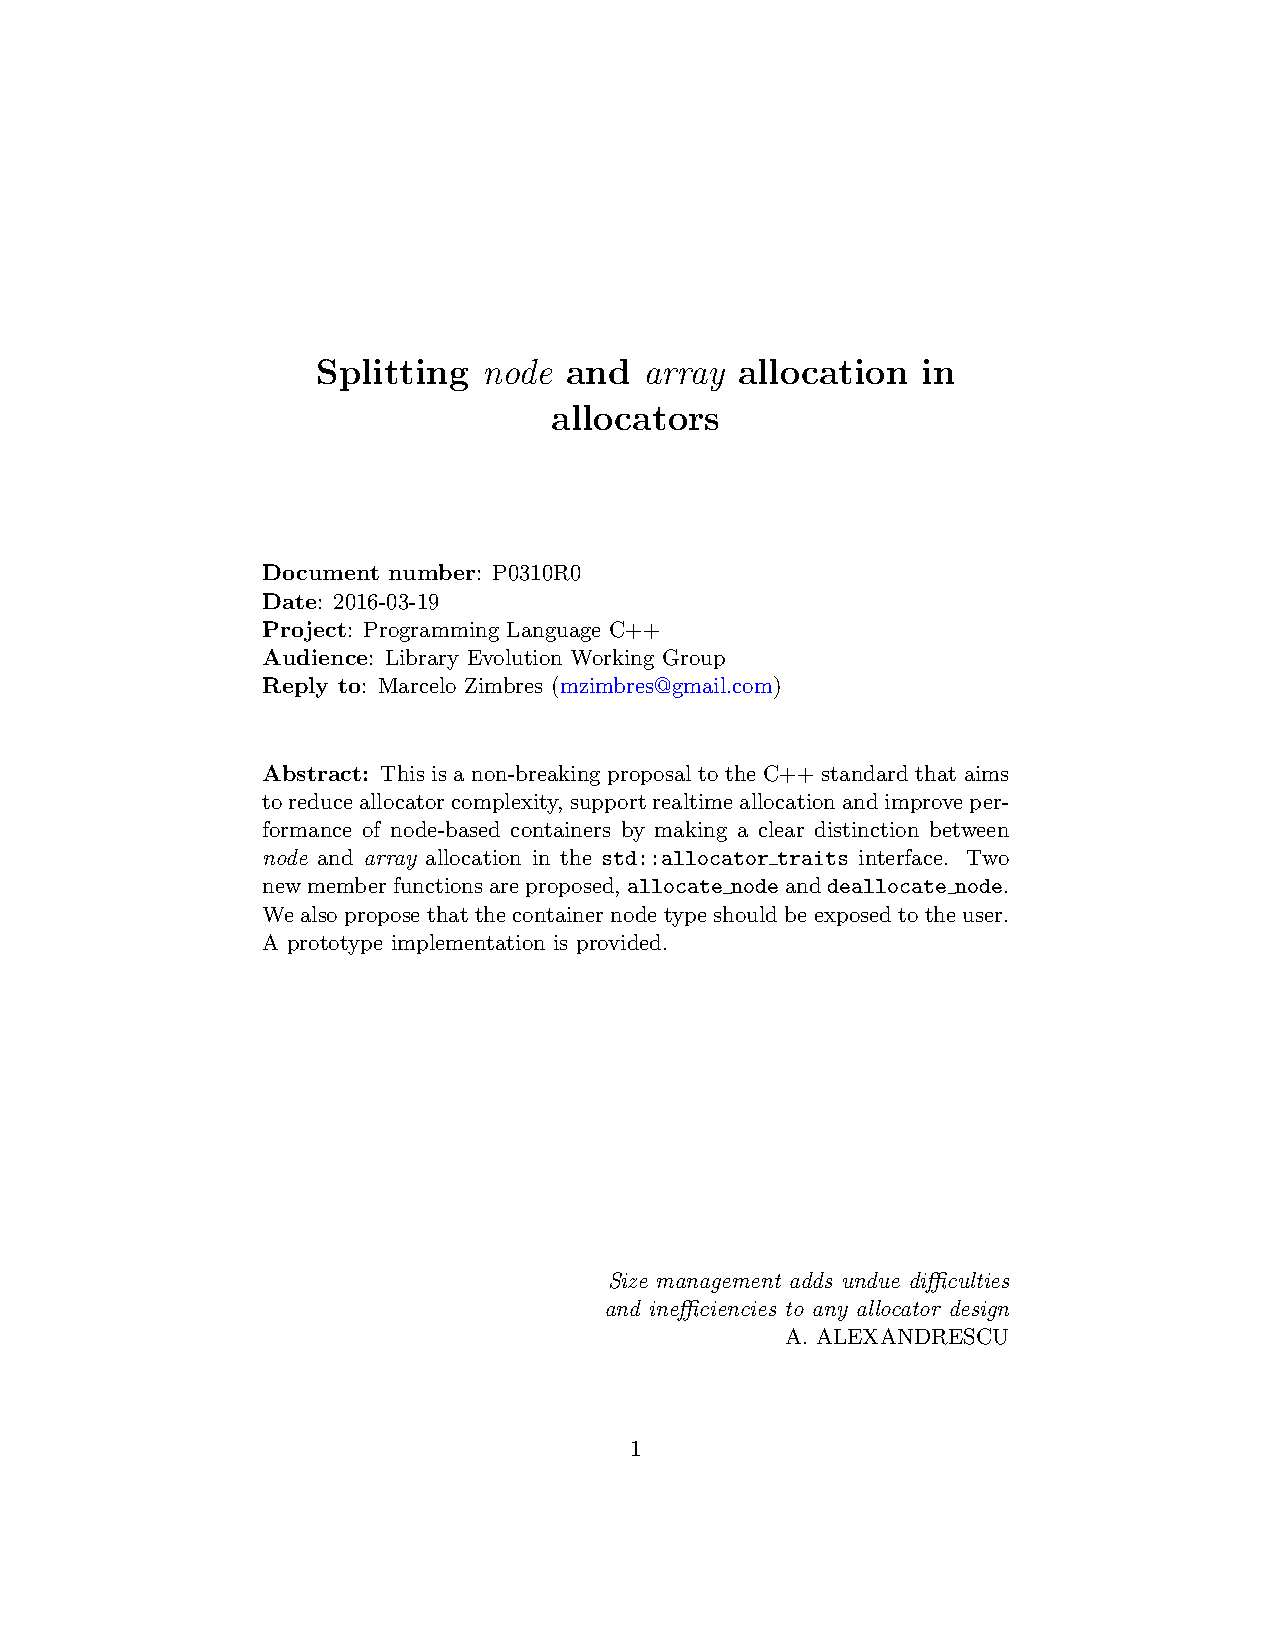
\includegraphics[scale=0.6]{fig/prop1.pdf} \\
    \end{center}
\end{frame}

\section{Node allocation}

\begin{frame}[fragile]{Containers and their allocation patterns}
\begin{columns}
\begin{column}{0.5\textwidth}

Node Allocation

\begin{itemize}
\item Simple and straighforward implementation.
\item Suitable for realtime/embedded.
\item Reduces memory fragmentation.
\item Basic building block used in array allocations as well.
\end{itemize}

\end{column}

\begin{column}{0.5\textwidth}
\begin{enumerate}
\item<alert@2> Get $N$ nodes at once.
\item<alert@3> Link them as a stack.
\item<alert@4> Repeat if more nodes are inserted.
\end{enumerate}

\end{column}
\end{columns}

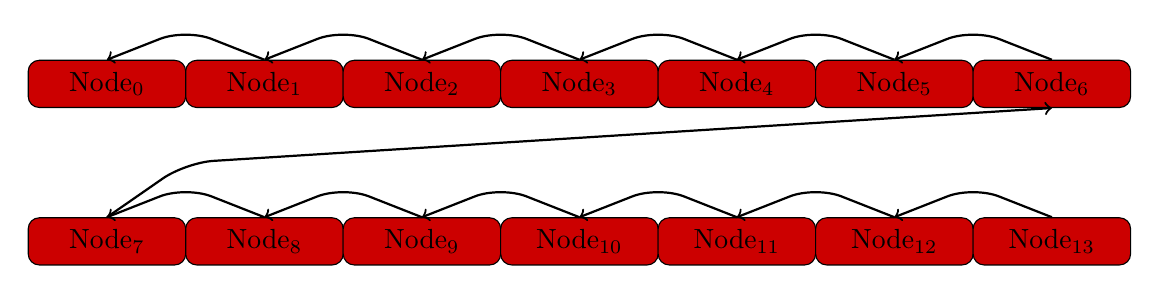
\begin{tikzpicture}[scale=1.0, rounded corners]

   \uncover<2-> {
      \dgfile (node0) at (-5.0,4) {Node$_0$};
      \dgfile (node1) at (-3.0,4) {Node$_1$};
      \dgfile (node2) at (-1.0,4) {Node$_2$};
      \dgfile (node3) at (1.0,4) {Node$_3$};
      \dgfile (node4) at (3.0,4) {Node$_4$};
      \dgfile (node5) at (5.0,4) {Node$_5$};
      \dgfile (node6) at (7.0,4) {Node$_6$};
   }

   \uncover<3-> {
      \draw[thick,<-,rounded corners=10pt,color=black] (node0.north) -- (-4,4.7) -- (node1.north);
      \draw[thick,<-,rounded corners=10pt,color=black] (node1.north) -- (-2,4.7) -- (node2.north);
      \draw[thick,<-,rounded corners=10pt,color=black] (node2.north) -- ( 0,4.7) -- (node3.north);
      \draw[thick,<-,rounded corners=10pt,color=black] (node3.north) -- ( 2,4.7) -- (node4.north);
      \draw[thick,<-,rounded corners=10pt,color=black] (node4.north) -- ( 4,4.7) -- (node5.north);
      \draw[thick,<-,rounded corners=10pt,color=black] (node5.north) -- ( 6,4.7) -- (node6.north);
   }

   \uncover<4-> {

      \dgfile (node7) at (-5.0,2) {Node$_{7}$};
      \dgfile (node8) at (-3.0,2) {Node$_{8}$};
      \dgfile (node9) at (-1.0,2) {Node$_{9}$};
      \dgfile (node10) at ( 1.0,2) {Node$_{10}$};
      \dgfile (node11) at ( 3.0,2) {Node$_{11}$};
      \dgfile (node12) at ( 5.0,2) {Node$_{12}$};
      \dgfile (node13) at ( 7.0,2) {Node$_{13}$};
   }

   \uncover<5-> {

      \draw[thick,<-,rounded corners=10pt,color=black] (node6.south) --  (-4,3) --  (node7.north);
      \draw[thick,<-,rounded corners=10pt,color=black] (node7.north) --  (-4,2.7) -- (node8.north);
      \draw[thick,<-,rounded corners=10pt,color=black] (node8.north) --  (-2,2.7) -- (node9.north);
      \draw[thick,<-,rounded corners=10pt,color=black] (node9.north) --  ( 0,2.7) -- (node10.north);
      \draw[thick,<-,rounded corners=10pt,color=black] (node10.north) -- ( 2,2.7) -- (node11.north);
      \draw[thick,<-,rounded corners=10pt,color=black] (node11.north) -- ( 4,2.7) -- (node12.north);
      \draw[thick,<-,rounded corners=10pt,color=black] (node12.north) -- ( 6,2.7) -- (node13.north);
   }
\end{tikzpicture}


\end{frame}

\begin{frame}[fragile]{Array Allocation}
Array allcation
\begin{itemize}
\item Many possible strategies. Which one should I use?
\item Has to handle different sizes.
\item No silver bullet. Every problem requires a different approach.
\item Users do not want to care about this unless there is need.
\item malloc: suitable for large memory blocks, overused, hundreds of
\item LOC, system calls, etc.
\item May use node allocation as a building block.
\end{itemize}

\end{frame}

\begin{frame}[fragile]{Underlying data structure}
\begin{columns}
\begin{column}{0.5\textwidth}
\begin{enumerate}
\item<alert@1> $N \le 256$ with $T \in [0, 256]$
\item<alert@2> $N \le 2^{16}$ with $T \in [0, 2^{16}]$
\item<alert@3> $N \le 2^{32}$ with $T \in [0, 2^{32}]$
\item<alert@4> $N \le 2^{64}$ with $T \in [0, 2^{64}]$
\end{enumerate}

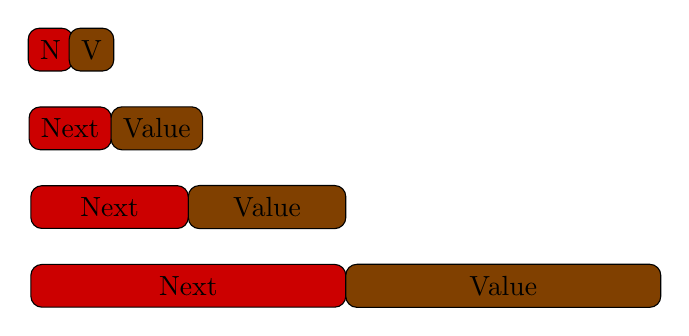
\begin{tikzpicture}[scale=1.0, rounded corners]

   \uncover<1-> {
      \nodeU (next) at (0.25,5) {N};
      \valueU (value) at (0.77,5) {V};
   }

   \uncover<2-> {
      \nodeD (next) at (0.5,4) {Next};
      \valueD (value) at (1.6,4) {Value};
   }

   \uncover<3-> {
      \nodeQ (next) at (1,3) {Next};
      \valueQ (value) at (3,3) {Value};
   }
   \uncover<4-> {
      \nodeO (next) at (2,2) {Next};
      \valueO (value) at (6,2) {Value};
   }
\end{tikzpicture}

\end{column}
\begin{column}{0.5\textwidth}

\begin{itemize}
\item The underlying data structure is a deque.
\item We do not have to address nodes with pointers.
\item For less than $256$ elements a \texttt{char} has enough bits.
\end{itemize}

\end{column}
\end{columns}

\end{frame}

\begin{frame}{Cache Hierarchy - Latency}{Why it is important to reduce memory usage}
    \begin{columns}
        \begin{column}{0.4\textwidth}
            Intel Haswell Mobile 
            \begin{itemize}
                \item Register: Fastest
                \item L0: 6 KiB
                \item L1: 128 KiB - 700 GiB/s
                \item L2: 1 MiB - 200 GiB/s
                \item L3: 6 MiB - 100 GB/s
                \item L4: 128 MiB - 40 GB/s
                \item Main memory – GiB - 10 GB/s
            \end{itemize}
        \end{column}

        %\begin{column}{0.6\textwidth}
        %    \begin{center}
        %        \includegraphics[scale=0.7]{fig/cache.jpg} \\
        %    \end{center}
        %\end{column}
    \end{columns}
\end{frame}

\begin{frame}[fragile]{Linked list travesal illustration}
\begin{enumerate}
\item<alert@1> Initial memory state
\item<alert@2> After awhile
\item<alert@2> Should we traverse the list chasing the pointers?
\item<alert@2> Or perhaps iterate sequentially though the whole
storage (deque) ignoring unused (red) nodes.
\item<alert@2> On heavily loaded storage traversing the later
can be much faster.
\end{enumerate}

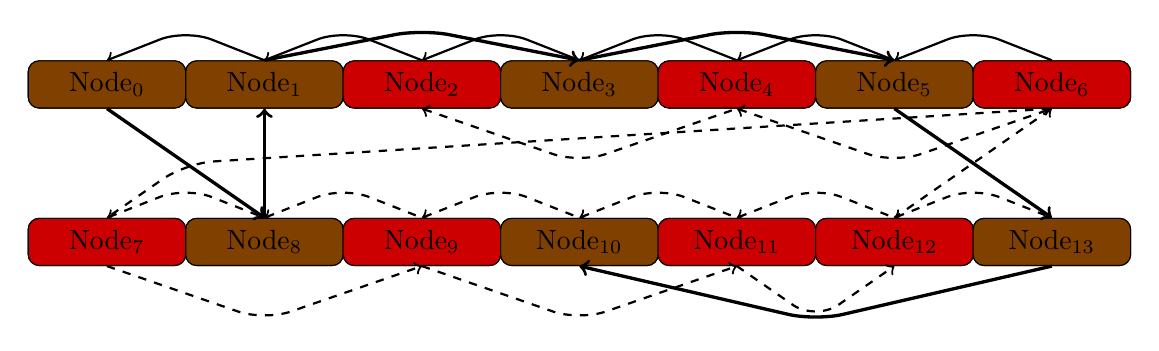
\begin{tikzpicture}[scale=1.0, rounded corners]

   \uncover<1> {
      \nodeQ (node0) at (-5.0,4) {Node$_0$};
      \nodeQ (node1) at (-3.0,4) {Node$_1$};
      \nodeQ (node2) at (-1.0,4) {Node$_2$};
      \nodeQ (node3) at (1.0,4) {Node$_3$};
      \nodeQ (node4) at (3.0,4) {Node$_4$};
      \nodeQ (node5) at (5.0,4) {Node$_5$};
      \nodeQ (node6) at (7.0,4) {Node$_6$};
      \nodeQ (node7) at (-5.0,2) {Node$_{7}$};
      \nodeQ (node8) at (-3.0,2) {Node$_{8}$};
      \nodeQ (node9) at (-1.0,2) {Node$_{9}$};
      \nodeQ (node10) at ( 1.0,2) {Node$_{10}$};
      \nodeQ (node11) at ( 3.0,2) {Node$_{11}$};
      \nodeQ (node12) at ( 5.0,2) {Node$_{12}$};
      \nodeQ (node13) at ( 7.0,2) {Node$_{13}$};

      \draw[thick,<-,rounded corners=10pt,color=black] (node0.north) -- (-4,4.7) -- (node1.north);
      \draw[thick,<-,rounded corners=10pt,color=black] (node1.north) -- (-2,4.7) -- (node2.north);
      \draw[thick,<-,rounded corners=10pt,color=black] (node2.north) -- ( 0,4.7) -- (node3.north);
      \draw[thick,<-,rounded corners=10pt,color=black] (node3.north) -- ( 2,4.7) -- (node4.north);
      \draw[thick,<-,rounded corners=10pt,color=black] (node4.north) -- ( 4,4.7) -- (node5.north);
      \draw[thick,<-,rounded corners=10pt,color=black] (node5.north) -- ( 6,4.7) -- (node6.north);


      \draw[thick,<-,dashed, rounded corners=10pt,color=black] (node6.south) --  (-4,3) --  (node7.north);
      \draw[thick,<-,dashed, rounded corners=10pt,color=black] (node7.north) --  (-4,2.7) -- (node8.north);
      \draw[thick,<-,dashed, rounded corners=10pt,color=black] (node8.north) --  (-2,2.7) -- (node9.north);
      \draw[thick,<-,dashed, rounded corners=10pt,color=black] (node9.north) --  ( 0,2.7) -- (node10.north);
      \draw[thick,<-,dashed, rounded corners=10pt,color=black] (node10.north) -- ( 2,2.7) -- (node11.north);
      \draw[thick,<-,dashed, rounded corners=10pt,color=black] (node11.north) -- ( 4,2.7) -- (node12.north);
      \draw[thick,<-,dashed, rounded corners=10pt,color=black] (node12.north) -- ( 6,2.7) -- (node13.north);
   }

   \uncover<2-> {
      \valueQ (node0) at (-5.0,4) {Node$_0$};
      \valueQ (node1) at (-3.0,4) {Node$_1$};
      \nodeQ (node2) at (-1.0,4) {Node$_2$};
      \valueQ (node3) at (1.0,4) {Node$_3$};
      \nodeQ (node4) at (3.0,4) {Node$_4$};
      \valueQ (node5) at (5.0,4) {Node$_5$};
      \nodeQ (node6) at (7.0,4) {Node$_6$};
      \nodeQ (node7) at (-5.0,2) {Node$_{7}$};
      \valueQ (node8) at (-3.0,2) {Node$_{8}$};
      \nodeQ (node9) at (-1.0,2) {Node$_{9}$};
      \valueQ (node10) at ( 1.0,2) {Node$_{10}$};
      \nodeQ (node11) at ( 3.0,2) {Node$_{11}$};
      \nodeQ (node12) at ( 5.0,2) {Node$_{12}$};
      \valueQ (node13) at ( 7.0,2) {Node$_{13}$};

      \draw[very thick,->,rounded corners=10pt,color=black] (node0.south) -- (node8.north);
      \draw[very thick,->,rounded corners=10pt,color=black] (node1.north) -- (-1,4.7) -- (node3.north);
      %\draw[thick,<-,rounded corners=10pt,color=black] (node2.north) -- ( 1,4.7) -- (node4.north);
      \draw[very thick,->,rounded corners=10pt,color=black] (node3.north) -- ( 3,4.7) -- (node5.north);
      %\draw[thick,<-,rounded corners=10pt,color=black] (node4.north) -- ( 4,4.7) -- (node5.north);
      \draw[very thick,->,rounded corners=10pt,color=black] (node5.south) -- (node13.north);
      %\draw[thick,<-,rounded corners=10pt,color=black] (node6.south) --  (-4,3) --  (node7.north);
      %\draw[thick,<-,rounded corners=10pt,color=black] (node7.north) --  (-4,2.7) -- (node8.north);
      \draw[very thick,->,rounded corners=10pt,color=black] (node8.north) -- (node1.south);
      %\draw[thick,<-,rounded corners=10pt,color=black] (node9.north) --  ( 0,2.7) -- (node10.north);
      %\draw[thick,<-,rounded corners=10pt,color=black] (node11.north) -- ( 4,2.7) -- (node12.north);
      %\draw[thick,<-,rounded corners=10pt,color=black] (node12.north) -- ( 6,2.7) -- (node13.north);
      \draw[very thick,->,rounded corners=10pt,color=black] (node13.south) -- (4,1.0) -- (node10.south);

      \draw[thick,<-,dashed, rounded corners=10pt,color=black] (node2.south) -- (1,3) -- (node4.south);
      \draw[thick,<-,dashed, rounded corners=10pt,color=black] (node4.south) -- (5,3) -- (node6.south);
      \draw[thick,<-,dashed, rounded corners=10pt,color=black] (node6.south) -- (node12.north);
      \draw[thick,->,dashed, rounded corners=10pt,color=black] (node11.south) -- (4,1)-- (node12.south);
      \draw[thick,->,dashed, rounded corners=10pt,color=black] (node9.south) -- (1,1)-- (node11.south);
      \draw[thick,->,dashed, rounded corners=10pt,color=black] (node7.south) -- (-3,1)-- (node9.south);
   }

\end{tikzpicture}

\end{frame}


\subsection[Node allocation]{Node allocation}
%\begin{frame}{Illustration}{Illustration}
%
%\begin{tikzpicture}[scale=1.0, rounded corners]
%
%   \uncover<1-> {
%      \dgfile (head) at (-5,4) {Head};
%   }
%   \uncover<2-> {
%      \dgfile (node1) at (-2,4) {Node$_1$};
%      \draw[thick,->,rounded corners=10pt,color=black] (head) -- (node1);
%   }
%   \uncover<3-> {
%      \dgfile (node2) at (1,4) {Node$_2$};
%      \draw[thick,->,rounded corners=10pt,color=black] (node1) -- (node2);
%   }
%   \uncover<4-> {
%      \dgfile (node3) at (4,4) {Node$_3$};
%      \draw[thick,->,rounded corners=10pt,color=black] (node2) -- (node3);
%   }
%   \uncover<5-> {
%      \dgfile (node4) at (7,4) {Node$_4$};
%      \draw[thick,->,rounded corners=10pt,color=black] (node3) -- (node4);
%   }
%\end{tikzpicture}
%
%\end{frame}

\section[Memory Usage]{Memory Usage}

%\begin{frame}{Size reduction}{Node sizes of \texttt{std::forward\_list<int>}}
%
%\begin{enumerate}
%\item<alert@1> $N \le 256$ with $T \in [0, 256]$
%\item<alert@2> $N \le 2^{16}$ with $T \in [0, 2^{16}]$
%\item<alert@3> $N \le 2^{32}$ with $T \in [0, 2^{32}]$
%\item<alert@4> $N \le 2^{64}$ with $T \in [0, 2^{64}]$
%\end{enumerate}
%
%\begin{tikzpicture}[scale=1.0, rounded corners]
%
%   \uncover<1-> {
%      \nodeU (next) at (0.25,5) {N};
%      \valueU (value) at (0.77,5) {V};
%   }
%
%   \uncover<2-> {
%      \nodeD (next) at (0.5,4) {Next};
%      \valueD (value) at (1.6,4) {Value};
%   }
%
%   \uncover<3-> {
%      \nodeQ (next) at (1,3) {Next};
%      \valueQ (value) at (3,3) {Value};
%   }
%   \uncover<4-> {
%      \nodeO (next) at (2,2) {Next};
%      \valueO (value) at (6,2) {Value};
%   }
%\end{tikzpicture}
%
%\end{frame}

\part{How to get node allocation in the STL}

\section[Implementation]{Implementation}
\begin{frame}<beamer>{Outline}
   \tableofcontents[currentsection,currentsubsection]
\end{frame}

\section[Proposal]{Proposal}
\section[Exposing the node type]{Exposing the node type}
\section[Node size reduction]{Node size reduction}
\section[Avoid pointer chasing]{Avoid pointer chasing}

\begin{frame}{Realtime node-based containers}
    \begin{columns}
        \begin{column}{0.5\textwidth}
            \texttt{std::unordered\_set}
            \begin{center}
                \includegraphics[scale=0.6]{fig/unordered_set_with_frag.pdf} \\
            \end{center}
        \end{column}

        \begin{column}{0.5\textwidth}
            \texttt{std::set}
            \begin{center}
                \includegraphics[scale=0.6]{fig/set_bench.pdf} \\
            \end{center}
        \end{column}
    \end{columns}
\end{frame}

\begin{frame}{}
    \vspace{1cm}
    \begin{center}
        {\Large \bf Thank you! Questions?} 
    \end{center}
\end{frame}

\end{document}


